\documentclass{article}

% if you need to pass options to natbib, use, e.g.:
%     \PassOptionsToPackage{numbers, compress}{natbib}
% before loading neurips_2020

% ready for submission
% \usepackage{neurips_2020}

% to compile a preprint version, e.g., for submission to arXiv, add add the
% [preprint] option:
%     \usepackage[preprint]{neurips_2020}

% to compile a camera-ready version, add the [final] option, e.g.:
%     \usepackage[final]{neurips_2020}

% to avoid loading the natbib package, add option nonatbib:
     \usepackage[nonatbib]{neurips_2020}

\usepackage[utf8]{inputenc} % allow utf-8 input
\usepackage[T1]{fontenc}    % use 8-bit T1 fonts
\usepackage{hyperref}       % hyperlinks
\usepackage{url}            % simple URL typesetting
\usepackage{booktabs}       % professional-quality tables
\usepackage{amsfonts}       % blackboard math symbols
\usepackage{nicefrac}       % compact symbols for 1/2, etc.
\usepackage{microtype}      % microtypography
\usepackage{graphicx}

% sec-5 results table
\begin{filecontents*}{data.json}
[
    {"firstName":"John", "lastName":"Doe"},
    {"firstName":"Anna", "lastName":"Smith"},
    {"firstName":"Peter", "lastName":"Jones"}
];
\end{filecontents*}

\title{11711: Reimplementing GoEmotions Baseline for Emotion Classification}

% The \author macro works with any number of authors. There are two commands
% used to separate the names and addresses of multiple authors: \And and \AND.
%
% Using \And between authors leaves it to LaTeX to determine where to break the
% lines. Using \AND forces a line break at that point. So, if LaTeX puts 3 of 4
% authors names on the first line, and the last on the second line, try using
% \AND instead of \And before the third author name.

\author{%
  Ethan Wu \\
  \texttt{yongyiw@andrew.cmu.edu} \\
  \And Yilin Wang \\
  \texttt{yilinwan@andrew.cmu.edu} \\
  \And Ziqi Liu \\
  \texttt{ziqil2@andrew.cmu.edu} \\
  % examples of more authors
  % \And
  % Coauthor \\
  % Affiliation \\
  % Address \\
  % \texttt{email} \\
  % \AND
  % Coauthor \\
  % Affiliation \\
  % Address \\
  % \texttt{email} \\
  % \And
  % Coauthor \\
  % Affiliation \\
  % Address \\
  % \texttt{email} \\
  % \And
  % Coauthor \\
  % Affiliation \\
  % Address \\
  % \texttt{email} \\
}

\begin{document}

\maketitle

% \section*{THIS IS NOT COMPLETED YET!}
% This section will be removed once the report is completed. 

% Link to Github repo: https://github.com/yongyi-wu/nlp-group

\section{Introduction}

Emotion recognition is a task essential for many tasks, from dialog systems construction to spam detection. Emotion classification, as a subbranch of emotion detection, focuses on assigning labels that could be easily understood by humans to given input texts. 

Our project was inspired by the \textit{GoEmotions} datasets (Demszky, 2020)\cite{main}. The main goal of this dataset is to produce a corpus using a more fine-grained emotion taxonomy than current Ekman's taxonomy. This paper also released a baseline emotion prediction model by fine-tuning BERT on their proposed dataset, achieving a macro-average F1-score of $.46$ across GoEmotion's taxonomy, leaving much room for improvement. As the dataset is relatively new, the baseline BERT model is also the state-of-the-art (SOTA) model. In this paper, BERT model finetuned on the proposed dataset shows transferability to other emotion predictions target datasets listed in \emph{an analysis of annotated corpora for emotion classification in text. } (Bostan \& Klinger, 2018) \cite{Unified}

We have made code and data related to the experiment reproduction available at: \href{https://github.com/yongyi-wu/nlp-group}{https://github.com/yongyi-wu/nlp-group}. 


\section{Literature Review}
\label{lit}

\subsection{Fundamental knowledge of the Emotion Recognition in Conversation (ERC) task}

\paragraph{Emotion taxonomy: } There are two types of emotion categorization in the field: categorical and dimensional. On the categorical front, Ekman's model divides emotions into 6 fundamental emotions (fear, disgust, surprise, joy, anger, sadness), while Plutchik's emotion wheels divide emotions into 8 fundamental types, with each being able to subdivide into subcategories. For dimensional approaches, emotion can be expressed continuously in two dimensions: valence (degree of positivity) and arousal (degree of intensity).

GoEmotions dataset extends this traditional taxonomy to $27$ subcategories (excluding neutral), allowing models to learn more fine-grained distinction between emotions in the corpora. 

\paragraph{Existing Datasets for emotion classification in text: } In \textit{An Analysis of Annotated Corpora for Emotion Classification in Text} (2018), Bostan and Klinger aggregated existing emotion classification corpora into a one framework with unified annotation schema and file format (In GoEmotions' paper, the author uses $9$ datasets mentioned in this paper as target datasets for their transferring learning experiments). The nine datasets are Daily Dialog \cite{dataset-DailyDialog}, Emotion Stimulus \cite{dataset-EmotionStimulus}, EmoInt \cite{dataset-EmoInt}, Electoral Tweets \cite{dataset-Electoral Tweets}, Affective Text \cite{dataset-Affective text}, ISEAR \cite{dataset-ISEAR}, CrowdFlower \cite{dataset-CrowdFlower}, TEC \cite{dataset-TEC}, SSEC \cite{dataset-SSEC}. All of the nine datasets have Ekman's annotation available excepts SSEC and Electoral Tweets, which uses Plutchik's annotations. 

\subsection{Emotion Recognition in Conversation (ERC)}
Emotion classification is the main task that the $GoEmotions$ dataset addresses. Emotion classification is a subtask of Emotion Recognition in Conversation (ERC), which involves dialogue data (multi-speaker, multiple utterances), where the model is given an entire conversation and is required to predict emotion labels for each utterance. Our main task, emotion classification, does not require an entire conversation as the input, but rather predicts emotion labels for a single Reddit comment. 

However, it is noteworthy that emotion classification and ERC share huge common ground, and many techniques used in ERC tasks can be adapted to emotion classification to improve model performance. Moreover, although the processed go-emotion dataset only contains sentence-level Reddit comments, the raw data do include links to the parent text. Therefore, it is possible to use GoEmotions in ERC settings, which will allow our model to use contextual information. In the rest of this section, we will examine literature that is relevant to emotion classification as well as to ERC. 

\subsection{Challenges in the fields}

In 2019, the paper \textit{Emotion Recognition in Conversation: Research Challenges, Datasets, and Recent Advances}\cite{survey2019} (Poria et al., 2019) surveys the challenge of emotion classification tasks and drawbacks in recent models and approaches. Here we listed a few relevant points associated with emotion classification. 

\paragraph{Sarcasm in dialog} Detection of sarcasm is important in emotion recognition, as literal interpretations of emotions will almost definitely fail when conversations involve sarcasm. 

\paragraph{Emotional reasoning} It is possible for each part of the text to contain different emotions. The model must be able to recognize emotions in different parts of the sentence and reason through them logically for it to understand sentence-level semantics, which is crucial for classification. 

\subsection{Drawbacks of current approaches and Contribution of GoEmotions}
\paragraph{Drawback of emotion model} Ekman's categorization is too simple and unable to ground complex emotions, Plutchik's emotion wheel model is hard for annotators to distinguish emotions are different intensities (e.g. rage and anger). Recent datasets such as DailyDialog only deploy Ekman's emotion annotations.

\paragraph{Contribution of GoEmotions} GoEmotions addresses the prior drawback by employing a 27-fold categorization of emotions. By including more complicated and subtle emotions like ``realization" and ``curiosity", we force the model to achieve a higher level of natural language understanding (NLU). If the model performs well in classifying complicated emotion, it must be able to perform better under simpler emotion taxonomies, like Ekman's model.  


\subsection{Related datasets and State-Of-The-Art (SOTA) models in Emotion Classification}
\label{related}

\subsubsection{Dataset: Affect in Tweets}
The SemEval-2018 Task 1: \textit{Affect in Tweets} is a dataset that contains annotated Tweets in English, Arabic, and Spanish. The dataset was created for the following 5 tasks 1) emotion intensity
regression, 2) emotion intensity ordinal classification, 3) valence regression 4) valence ordinal classification and 5) emotion classification. For the emotion classification task, each tweet is annotated with one of the 12 emotions (including neutral) by multiple annotators, and the annotations were aggregated so that each tweet may receive multiple labels. 

\paragraph{SpanEmo} The SOTA model on \textit{Affect in Tweets}, achieving a multi-label accuracy of 0.601 and macro F1-score of 0.578 on the English dataset. Consider over-lap of emotions within sentences. Cast multi-label emotion prediction into a span prediction problem. Aid ER (Emotion Recognition) model to associate labels with words in a sentence. (Potential direction for A4. From single-label emotion prediction to multi-label emotion prediction.)

\paragraph{BERT+DK} In \textit{Improving Multi-label Emotion Classification by Integrating both General and Domain-specific Knowledge} (Ying et al., 2019), the authors first finetuned BERT on twitter sentences to learn general linguistic knowledge, and they utilized a Twitter-specific text preprocessor (\textit{ekphrasis}, Baziotis et al., 2017) to include domain-specific knowledge into the representation. 

\subsubsection{Dataset: ROCStories}
ROCStories contains 50K 5-sentence stories that capture the causal and commonsense relations between daily events. Rashkin et al. annotated a subset of ROCStories with one or more of the eight emotion labels for each story.

\paragraph{Semi-supervision} Gaonkar et al. found that adding the pretrained label semantics embeddings as input and incorporating the learned correlation between emotions in the loss function improves the performance over the baseline BERT model. Augmenting this method and applying semi-supervised techniques on the unlabeled portion of ROCStories gives the SOTA model with F1-score being 65.88, which is 4.92 point higher than the baseline BERT model. 

\subsubsection{Dataset: DailyDialog} DailyDialog collects human dyadic (two-party dialog) daily conversation as data, and deploys Ekman's emotion model for emotion annotation. This dataset does not annotate the speaker's name for each utterance.

\paragraph{CESTa} In \textit{Contextualized Emotion Recognition in Conversation as Sequence Tagging} (Wang et al., 2020) \cite{CESTa}, Wang et al. were the first to cast ERC task to sequence tagging task. They used CRF to model the emotional consistency within context to find the best tag sequence for the entire conversation. They remain the SOTA result on the DailyDialog dataset. 

\subsubsection{Dataset: IEMOCAP} IEMOCAP is a multi-modal, dyadic (two-party) dialogue dataset, collected from 10 participant's conversations. IEMOCAP has about 5 times more utterances per dialogue than MELT. IEMOCAP doesn't assign speaker names

\paragraph{EmoBERTa} In \textit{EmoBERTa: Speaker-Aware Emotion Recognition in Conversation with
RoBERTa} (Kim \& Vossen, 2021) \cite{EmoBERTa} finetunes RoBERTa-large model on IEMOCAP and MELD datasets and achieves SOTA results respectively. Their creativity lies at the appending future utterances to the inputs into the RoBERTa model (three-segmented input, past utterances appending current utterances appending future utterances), and prepending speaker's name before each utterance, so that RoBERTa becomes speaker-aware, and hence able to model self and inter-personal emotional influences. 

\subsubsection{MELD} MELD is a multi-model, multi-party dataset derived from dialogues in TV series \textit{Friends}. MELD's emotional class distribution is highly imbalanced, and hence a lot of model uses the weight-F1 score to measure model performance when trained on this dataset. MELD assigns speakers' names to each utterance.

\paragraph{TODKAT} In \textit{Topic-Driven and Knowledge-Aware Transformer for Dialogue Emotion Detection} (Lixing Zhu, Gabriele Pergola, Lin Gui, Deyu Zhou, Yulan He), the author proposes the first topic-driven approach to the ERC task. They use an augmented LM for topic detection, and retrieve commonsense the knowledge from knowledge base based on conversational context. The fused representation and then fed into a Transformer encoder-decoder model to derive the emotion labels for every utterance. 


\section{Reimplementation Details}

In our assignment 3 project, we rerun the fine-tune training of the paper's model (BERT base) on GoEmotions dataset, and produce similar scores. Based on Table 1, 2, and 3, our results (precision, recall, F1) are within the standard deviation of the reference results. In fact, our results differ from the reference by a very small amount, which is much less than the std. 

We also rerun the transfer learning experiments in section 6 of the original paper and redraw the 9 plots of their results. See results in Figure \ref{fig:sec6}.

\begin{figure}[ht]
    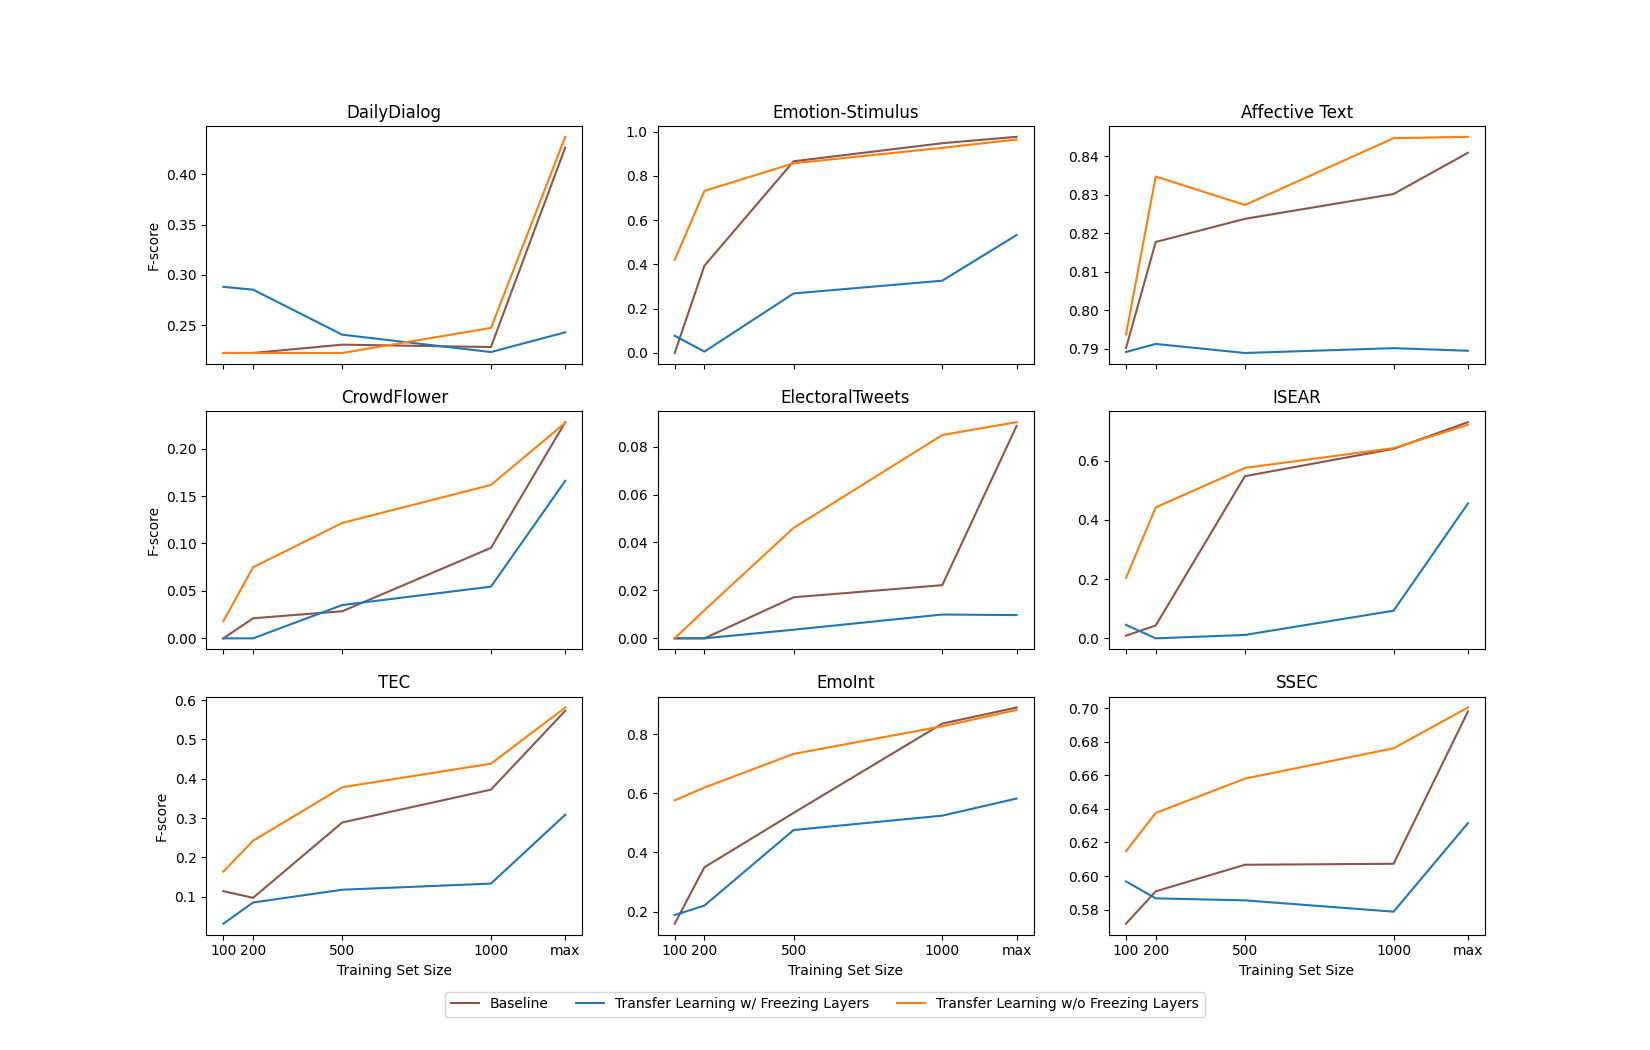
\includegraphics[width=\textwidth]{section6_f1.png}
    \centering
    \caption{Transfer learning performance on 9 datasets}
    \label{fig:sec6}
\end{figure}

%\begin{figure}[h!]
\begin{minipage}[c]{0.55\textwidth}
\centering
{Table 1: Results based on GoEmotions taxonomy}
\begin{tabular}{c c c c}
\hline\hline
Emotion & Precision & Recall & F1 \\ [0.5ex]
\hline 
admiration & 0.633 & 0.738 & 0.681\\
amusement & 0.750 & 0.909 & 0.822\\
anger & 0.493 & 0.525 & 0.509\\
annoyance & 0.342 & 0.431 & 0.381\\
approval & 0.398 & 0.459 & 0.426\\
caring & 0.440 & 0.459 & 0.449\\
confusion & 0.362 & 0.516 & 0.426\\
curiosity & 0.490 & 0.658 & 0.562\\
desire & 0.583 & 0.506 & 0.542\\
disappointment & 0.331 & 0.351 & 0.341\\
disapproval & 0.366 & 0.431 & 0.396\\
disgust & 0.483 & 0.463 & 0.473\\
embarrassment & 0.600 & 0.405 & 0.484\\
excitement & 0.429 & 0.466 & 0.447\\
fear & 0.588 & 0.769 & 0.667\\
gratitude & 0.920 & 0.912 & 0.916\\
grief & 0.000 & 0.000 & 0.000\\
joy & 0.539 & 0.646 & 0.588\\
love & 0.745 & 0.870 & 0.802\\
nervousness & 0.381 & 0.348 & 0.364\\
optimism & 0.552 & 0.602 & 0.576\\
pride & 0.667 & 0.125 & 0.211\\
realization & 0.246 & 0.200 & 0.221\\
relief & 0.000 & 0.000 & 0.000\\
remorse & 0.584 & 0.804 & 0.677\\
sadness & 0.549 & 0.571 & 0.560\\
surprise & 0.545 & 0.553 & 0.549\\
neutral & 0.630 & 0.672 & 0.651\\
\textbf{macro-average} & \textbf{ 0.487 } & \textbf{ 0.514 } & \textbf{ 0.490 }\\
\textbf{std (ref)} & \textbf{0.18} & \textbf{ 0.24} & \textbf{ 0.19 }\\[1ex] 
\hline 
\end{tabular}

%\vspace{-25ex}
%\newline


\end{minipage}
\begin{minipage}[c]{0.55\textwidth}
{Table 2: Results based on sentiment-grouped data.}
\centering
\begin{tabular}{c c c c}
\hline\hline
Emotion & Precision & Recall & F1 \\ [0.5ex]
\hline 
ambiguous & 0.511 & 0.645 & 0.570\\
negative & 0.639 & 0.727 & 0.680\\
positive & 0.765 & 0.855 & 0.807\\
\textbf{macro-average} & \textbf{ 0.639 } & \textbf{ 0.723 } & \textbf{ 0.678 } \\ 
\textbf{std (ref)} & \textbf{0.09} & \textbf{0.10} & \textbf{0.09}\\[1ex] 
\hline 
\end{tabular}

%\vspace{10ex}
\vspace{20ex}

{Table 3: Results based on Ekman taxonomy.}
\centering
\begin{tabular}{c c c c}
\hline\hline
Emotion & Precision & Recall & F1 \\ [0.5ex]
\hline 
anger & 0.502 & 0.574 & 0.536\\
disgust & 0.470 & 0.512 & 0.490\\
fear & 0.612 & 0.724 & 0.664\\
joy & 0.783 & 0.860 & 0.819\\
sadness & 0.556 & 0.604 & 0.579\\
surprise & 0.523 & 0.662 & 0.584\\
\textbf{macro-average} & \textbf{ 0.583 } & \textbf{ 0.658 } & \textbf{ 0.618 } \\ 
\textbf{std (ref)} & \textbf{0.10} & \textbf{0.11} & \textbf{0.10}\\[1ex] 
\hline 
\end{tabular}
\end{minipage}
%\end{figure}



\section{Error analysis}
In Table 2, we see that our model performs the best on positive emotions and worst on ambiguous emotions. More specifically, Table 1 shows that our model performs particularly badly in classifying emotions such as ``realization", ``pride", and ``annoyance". A plausible explanation is that these emotions are more complicated and require more contextual information to properly classify. 

As described above, GoEmotions characterizes a multi-label classification task. Our model performs this task by producing a probability measure for different labels for each sample. We use an aggregation procedure so that our prediction retains at most 3 labels for each sample. 

For the sake of simplicity, we use the following procedures in later error analysis. If the sample contains only has 1 true label, then it is considered correctly classified if the top 1 predicted label is the same as the true label. If the sample contains multiple true labels, it is considered correct if all its label is contained in the top 3 predicted label. 

Table 4 and 5 provide some most common mistakes made by our model using the GoEmotions classifications of emotion. We see in table 4 that the most common errors for single-label samples can be generalized as the misclassification between ``neutral" and positive/negative emotion labels. We see in table 5 that for samples with multiple labels, our model often succeed in predicting one of the labels (which refers to simpler emotions such as ``neutral" or ``love"), but fail to recognize more complicated emotions (like ``realization" and ``annoyance"). 


\begin{table}[h!]
\renewcommand\thetable{4}
\caption{Top 7 common error for samples with only 1 true label}
\centering
\begin{tabular}{l  l  l }
\hline\hline
True Label& Predicted Label & Occurrence  \\ [0.5ex]
\hline 
neutral  & approval  & 89\\
neutral  & disapproval  & 72\\
neutral  & curiosity  & 68\\
approval  & neutral  & 67\\
neutral  & annoyance  & 61\\
disapproval  & neutral  & 56\\
annoyance  & neutral  & 55\\[1ex]
\hline 
\end{tabular}
\label{table:nonlin} 
\end{table}

In table 6 we present 2 typical misclassified examples that are perhaps indicative of how the error is made. It is plausible to argue that the classifier did not achieve a high understanding of the semantics of the sentence, but it utilizes only certain characteristics of the sentence to make the classification. For example, the reason that sentence (A) is classified as ``annoyance" is probably because it contains the word ``moron", which is usually indicative of annoyance or anger. Similarly,  the reason that sentence (B) is classified as ``curious" is probably that contains``?", which is usually indicative of curiosity. However, in (A) and (B), the presence of these two words does not mean that the sentence exhibit other emotion other than ``neutral". 

Therefore, it is plausible to say that the BERT model did not achieve a high level of natural language understanding (NLU). The use of a more advanced NLU model that incorporates semantics is necessary to improve the model performance. 


\begin{table}[h!]
\renewcommand\thetable{5}
\caption{Top 5 common error for samples with multiple true label}
\centering
\begin{tabular}{l  l  l l}
\hline\hline
True Label 1& True Label 2&Predicted Label & Occurrence  \\ [0.5ex]
\hline 
annoyance & neutral  & neutral  & 10\\
approval& neutral  & neutral  & 8\\
admiration& love  & love  & 7\\
approval &admiration  & admiration  & 7\\
realization& neutral  & neutral  & 6\\
annoyance& disapproval  & neutral  & 5\\
[1ex]
\hline 
\end{tabular}
\label{table:nonlin} 
\end{table}

\begin{table}[h!]
\renewcommand\thetable{6}
\caption{Two representative mistakes}
\centering
\begin{tabular}{l  l  l l l} \hline \hline 
ID &Sentence & True Label& Predicted Label  \\ [0.5ex]
\hline
(A)& That's a very long way of saying "I'm a moron"  & anger  & annoyance\\[1ex]
(B) &You know that mista mista lady? I think I just killed her. - [NAME] & neutral  & curiosity\\[1ex]
\hline 
\end{tabular}
\label{table:nonlin} 
\end{table}






\section{Further Improvements}
In section 4, we argued that our model did not achieve a high level of natural language understanding and we need to use more advanced NLU models. To address this issue, we could use some SOTA NLU models such as HNN (He et al.) \cite{HNN} in future work. 

In Section 4, we also see that our model often fails to distinguish ``neutral" from other emotions. To address this issue, it may be helpful to use contrastive learning in our model to force the model to separate (embedding of words) ``neutral" from other emotions. For example, in finetuning, we could include contrastive learning objectives in the loss function, as suggested by Gunel et al. (2021) \cite{CLMFT}. It is also possible to adapt existing pretrained language models that were trained on contrastive learning objectives, such as CERT (Fang et al., 2020) \cite{CERT}. 

The work by Gaonkar et al., which highlights the importance of the label semantics, also appears to be a promising direction in the emotion classification task. This is because incorporating label semantics enables us to avoid treating each category independently but leverage inherent distance within and across positive, neutral ,and negative emotions. Therefore, we can consider replacing the label token with label embedding, including the label embedding as inputs, and taking label correlation into account in the loss function. These modifications can potentially address the aforementioned vulnerabilities of the baseline model. 


\newpage

\begin{thebibliography}{9}
\bibitem{main}
Dorottya Demszky, Dana Movshovitz-Attias, Jeongwoo Ko, Alan Cowen, Gaurav Nemade, and Sujith Ravi (2020). \emph{GoEmotions: A Dataset of Fine-Grained Emotions}, arXiv:2005.00547 [cs.CL].

\bibitem{dataset-DailyDialog}
Li Yanran, Su Hui, Shen Xiaoyu, Li Wenjie, Cao Ziqiang, and Niu Shuzi (2017). \emph{DailyDialog: A Manually Labelled Multi-turn Dialogue Dataset}, Proceedings of the Eighth International Joint Conference on Natural Language Processing (Volume 1: Long Papers), Asian Federation of Natural Language Processing.

\bibitem{dataset-EmotionStimulus}
Diman Ghazi, Diana Inkpen, and Stan Szpakowicz.
(2015). \emph{Detecting Emotion Stimuli in EmotionBearing Sentences}. In International Conference on Intelligent Text Processing and Computational Linguistics, pages 152–165. Springer.

\bibitem{dataset-Affective text}
Carlo Strapparava and Rada Mihalcea (2007). \emph{SemEval2007 task 14: Affective text}. In Proceedings of the Fourth International Workshop on Semantic Evaluations (SemEval-2007), pages 70–74, Prague, Czech Republic. Association for Computational Linguistics.

\bibitem{dataset-Electoral Tweets}
Saif M Mohammad, Xiaodan Zhu, Svetlana Kiritchenko, and Joel Martin (2015). \emph{Sentiment, emotion, purpose, and style in electoral tweets}. Information Processing & Management, 51(4):480–499.

\bibitem{dataset-ISEAR}
Klaus R Scherer and Harald G Wallbott (1994). \emph{Evidence for Universality and Cultural Variation of Differential Emotion Response Patterning}. Journal of personality and social psychology, 66(2):310.

\bibitem{dataset-CrowdFlower}
CrowdFlower (2016). https://www.figureeight.com/data/sentiment-analysis-emotion-text/.

\bibitem{dataset-TEC}
Saif M Mohammad (2012). \# emotional tweets. \emph{In Proceedings of the First Joint Conference on Lexical
and Computational Semantics-Volume 1: Proceedings of the main conference and the shared task, and
Volume 2: Proceedings of the Sixth International
Workshop on Semantic Evaluation}, pages 246–255.
Association for Computational Linguistics.

\bibitem{dataset-EmoInt}
Saif Mohammad, Felipe Bravo-Marquez, Mohammad
Salameh, and Svetlana Kiritchenko (2018). \emph{SemEval2018 task 1: Affect in tweets}. In Proceedings of The 12th International Workshop on Semantic Evaluation, pages 1–17, New Orleans, Louisiana. Association for Computational Linguistics.

\bibitem{dataset-SSEC}
Hendrik Schuff, Jeremy Barnes, Julian Mohme, Sebastian Pado, and Roman Klinger (2017). \emph{Annotation, ´
modelling and analysis of fine-grained emotions on
a stance and sentiment detection corpus}. In Proceedings of the 8th Workshop on Computational Approaches to Subjectivity, Sentiment and Social Media Analysis, pages 13–23.

\bibitem{BERT}
Jacob Devlin, Ming-Wei Chang, Kenton Lee, and
Kristina Toutanova (2019). \emph{Bert: Pre-training of deep bidirectional transformers for language understanding}. In 17th Annual Conference of the North American Chapter of the Association for Computational
Linguistics (NAACL).

\bibitem{Unified}
Laura-Ana-Maria Bostan and Roman Klinger (2018).
\emph{An analysis of annotated corpora for emotion classification in text}. In Proceedings of the 27th International Conference on Computational Linguistics,
pages 2104–2119.

\bibitem{survey2019}
Soujanya Poria, Navonil Majumder, Rada Mihalcea, Eduard Hovy (2019). \emph{Emotion Recognition in Conversation: Research Challenges, Datasets, and Recent Advances}. arXiv:1905.02947.

\bibitem{CMN}
D. Hazarika, S. Poria, A. Zadeh, E. Cambria, L.-P.
Morency, and R. Zimmermann (2018). \emph{Conversational memory network for emotion recognition in dyadic dialogue videos}. Proceedings of the 2018 Conference of the North American Chapter of the Association for Computational Linguistics: Human Language Technologies,
Volume 1 (Long Papers), vol. 1, 2018, pp. 2122–2132.

\bibitem{ICON}
D. Hazarika, S. Poria, R. Mihalcea, E. Cambria, and
R. Zimmermann (2018). \emph{Icon: Interactive conversational memory network for multimodal emotion detection}. Proceedings of the 2018 Conference on Empirical Methods in Natural Language Processing, 2018, pp. 2594–2604.

\bibitem{EmoBERTa}
Taewoon Kim, Piek Vossen (2021). \emph{EmoBERTa: Speaker-Aware Emotion Recognition in Conversation with RoBERTa}. arXiv:2108.12009. 

\bibitem{CESTa}
Wang Yan, Zhang Jiayu, Ma Jun, Wang Shaojun, Xiao Jing (2020). \emph{Contextualized Emotion Recognition in Conversation as Sequence Tagging}. Proceedings of the 21th Annual Meeting of the Special Interest Group on Discourse and Dialogue, Association for Computational Linguistics.  

\bibitem{TODKAT}
Lixing Zhu, Gabriele Pergola, Lin Gui, Deyu Zhou, Yulan He (2021). \emph{Topic-Driven and Knowledge-Aware Transformer for Dialogue Emotion Detection}. arXiv:2106.01071.

\bibitem{HNN}
Pengcheng He, Xiaodong Liu, Weizhu Chen, Jianfeng Gao (2019). \emph{A Hybrid Neural Network Model for Commonsense Reasoning}. arXiv:1907.11983. 

\bibitem{CERT}
Hongchao Fang, Sicheng Wang, Meng Zhou, Jiayuan Ding, Pengtao Xie (2020). \emph{CERT: Contrastive Self-supervised Learning for Language Understanding}. 	arXiv:2005.12766.

\bibitem{CLMFT}
Beliz Gunel, Jingfei Du, Alexis Conneau, Ves Stoyanov (2021). \emph{Supervised Contrastive Learning for
Pre-trained Language Model Fine-tuning.} 	arXiv:2011.01403. 
\end{thebibliography}
\newpage




\end{document}